% http://www.miccai2013.org/submission_guideline.html
\documentclass{llncs}

\usepackage{amsmath}
\usepackage{makeidx}
\usepackage[pdftex]{graphicx}
\usepackage{subfigure}

\def\wrt{w.\,r.\,t.}
\def\eg{e.\,g.}
\def\ie{i.\,e.}
\def\Dash{\nobreak\,---\penalty-500\,}

%%% Comments
\usepackage{color}
\newcommand{\TG}[1]{{\color{blue}\textbf{TG: #1}}}
\newcommand{\CD}[1]{{\color{green}\textbf{CD: #1}}}
\newcommand{\IP}[1]{{\color{cyan}\textbf{IP: #1}}}
\newcommand{\TODO}[1]{{\color{red}\textbf{TODO: #1}}}
%%%

\renewcommand{\Vec}[1]{\mathbf{#1}}
\newcommand{\Mat}[1]{\mathbf{#1}}

\begin{document}
%
%\frontmatter          % for the preliminaries
%
\mainmatter              % start of the contributions
%
\title{Complete Real-Time Liver Model Including Glisson's Capsule, Vascularization and Parenchyma}
%
\titlerunning{Complete Liver Model}  % abbreviated title (for running head)
%                                     also used for the TOC unless
%                                     \toctitle is used
%
\author{Anonymous}
%\author{%
%Tom\'a\v{s} Golembiovsk\'y\inst{1,2} \and%
%Igor Peterl\'ik\inst{3} \and%
%Christian Duriez\inst{2,4} \and%
%Stephan\'e Cotin\inst{2}%
%}
%
%\authorrunning{Tom\'a\vs Golembiovsk\'y et al.} % abbreviated author list (for running head)
%
%\institute{%
%Faculty of Informatics, Masaryk University, Brno, Czech Republic\and%
%INRIA Lille -- Nord, France\and%
%Institut Hospitallo-Universitaire, Strasbourg, France \and%
%University of Lille, Lille, France%
%}
%
\maketitle

\begin{abstract}
The accurate mechanical modeling of liver is of a paramount interest in simulation-based operation planning 
and computer-aided per-operative guidance. However, the realistic simulation of liver behaviour is a challenging task, 
since the organ is composed of three constituents: parenchyma, vascularization and Glisson's capsule, each having different mechanical properties. While the 
mechanical role of vessels on both global and local behaviour of the organ has been measured and modelled previously~\cite{Peterlik2012}, only local 
effects have been studied in the case of Glisson's capsule~\cite{Hollenstein2006,Ahn2010}. 

In this paper we introduce what we believe is the first real-time model of liver taking into account all three constituents, each being simulated with 
a different type of finite elements.
Using the model, we focus on the role of the Glisson's capsule: first, we show that the model is able to reproduce correctly
the local effects of the capsule in so called aspiration test. Second, based on CT image data of porcine abdominal cavity acquired in supine and flank 
positions, we demonstrate 
that the capsule has also a global impact on the mechanical behaviour of the liver in the case when the organ undergoes large deformations. 

%This work provides a complete physical model for the deformations of the liver with its three constituents: parenchyma, vessels and the Glisson's capsule.
%Some recent experimental results \cite{Ahn2010} have shown that there is a significant difference of stiffness between the Glisson's capsule and the parenchyma. 
%Moreover, it has been observed that the capsule plays an important role for the deformation at the local level \cite{Hollenstein2006}.
%However, the Glisson's capsule is very thin and its influence for the global deformations of the liver was never highlighted.
%In this work, we propose to use a membrane FEM model for the capsule, that is coupled with a vascularized model of the liver.
%We show that the approach is able to reproduce the deformations observed at the local level.
%Additionally, we show, by simulating natural global deformations of the liver observed on real images (due to gravity), that the results have important differences with and without the capsule.

\keywords{deformable liver model, Glisson's capsule, vascularization, real-time soft tissue modeling}
\end{abstract}

\section{Introduction} 
According to the statistics, nearly 100,000 European citizens die of cirrhosis or liver cancer each year. 
Although new methods such as radio-frequency- or cryo-ablation used in the interventional radiology 
seems to be promising, surgery remains the option that offers the foremost success rate against these pathologies. 
Nevertheless, surgery is not always performed due to several limitations, in particular the determination 
of accurate eligibility criteria for the patient. 
In this context, the pre-operational planning becomes a crucial task having a significant impact on the treatment. 

Computer-aided physics-based medical simulation has proven to be an extremely useful technique in the area of medical training. 
Nevertheless, whereas generic models are usually required in training simulators, accurate patient-specific modelling
becomes necessary as soon as computer simulation is to be employed in the pre-operative planning. At the same time, 
interactivity of such models remains an important aspect, requiring real-time simulation which is often difficult to 
achieve given the complexity of soft tissues. 

In case of human liver, the task of real-time accurate modeling is challenging, mainly because of the complex structure 
of this organ composed of three main constituents: \emph{parenchyma}, \emph{vascular networks} and \emph{Glisson's capsule}.
The parenchyma has certainly been the most studied component of the liver; today researchers agree on hyperelastic 
properties of the tissue, for which the mechanical parameters have been reported for example in~\cite{Kerdok2006,Gao2009}. 
Several methods have been proposed to model the hyperelastic behaviour at real-time rates, such as multiplicative Jacobian decomposition
introduced in~\cite{Marchesseau2010}.

The mechanical importance of the vascular structures in liver is studied in~\cite{Peterlik2012}. It shows that the 
influence of vessels on the mechanical behaviour of the organ is significant, mainly if large deformations occur. 
Since a detailed modeling of the vessels would be extremely costly (mainly because of the small thickness of the vessel wall, 
the authors propose a composite model allowing for real-time simulation of entire liver with vasculature.

Rather a small number of studies have been conducted on the last liver constituent, the  Glisson's capsule.
Quantitative results of experiments on a porcine liver have been published in~\cite{Umale2011}; the measurements indicate that although being very 
thin (10--20$\mu m$), the capsule shows to be stiff in tensile tests: the Young's modulus of the capsule (reported as $8.22\pm3.42$\,MPa) 
exceeds the values for the parenchyma by three orders of magnitude.
This suggests that the mechanical influence of the membrane on the liver behaviour is not negligible.

In~\cite{Hollenstein2006}, a local influence of the capsule has been measured using a special aspiration device. The study was then repeated 
in vivo on human patients during the operation, confirming the mechanical importance of the membrane~\cite{Ahn2010,Nava2008}.
To our best knowledge, no attempt has been made to demonstrate the role of the Glisson's capsule on the global behaviour of 
the liver, mainly if the organ undergoes large deformations which is often the case during the surgery.

The main contribution of the paper is twofold: first, we present an efficient real-time model of the liver, taking into account 
the parenchyma, vascularization and Glisson's capsule. The model is based on three different finite element representations for each constituent,
linked together via mechanical coupling. We show that the model mimics the \emph{local} experiments described in~\cite{Hollenstein2006}.
 
Second, we use the complete model of the liver to demonstrate the \emph{global} influence of the Glisson's
capsule via simulation: using a specific model of a porcine liver built from CT contrast-enhanced data, we show that there is a significant 
difference in the response of the model with and without the capsule in case when the liver undergoes large deformations. 

The paper is organized as follows: first we describe the proposed vascularized
liver model with capsule. Second, we validate our model in context of local deformations by reproducing the aspiration test 
described in~\cite{Hollenstein2006}. Finally, we demonstrate that in spite of it's small thickness, the Glisson's 
capsule has a global influence on the liver undergoing large deformations. 

%Then we show the correct behaviour of the
%model in context of \emph{local} deformations and finally we analyze the influence of
%the capsule on the \emph{global} deformations of the liver and show that despite the
%small thickness it plays an important role also in the \emph{global} context.


%Medical simulation is expected to play an integral part in many aspects of
%medical practice. From diagnosis, through planning or training to computer
%assisted intervention.
%Medical training application, like the ones for training laparoscopic
%surgery, have to operate in real-time and a good medical model has to be
%simple yet efficient to be really usable in this environment.
%
%Liver is largest internal organ formed mostly by a soft tissue (parenchyma)
%that is hyper-elastic and also visco-elastic. The parenchyma is interwoven
%by dense vascular network, this tree-like tubular structure is stiffer then
%the parenchyma. Finally the parenchyma is covered by very stiff collagenous
%membrane that preserves the integrity of the organ.
%
%Strangely, most of the work on liver modelling only considers the
%parenchyma and model the liver as single homogeneous object \TG{Refs}.
%Only recently
%Peterl\'{i}k et al. \cite{Peterlik2012} showed the importance of the vascular
%structures on the liver deformation.
%
%Another overlooked component is the Glisson's capsule.
%Biomechanical measurements report that the capsule has very small
%thickness (approx. 20 $\mu$m for porcine liver \cite{Umale2011}).
%On the other hand it has in three orders of magnitude higher stiffness than
%the parenchyma.
%Because of this it plays an important role in local
%deformations of the liver \cite{Ahn2010,Hollenstein2006}.
%It was reported that evaluation of the liver as a homogeneous material
%without capsule can lead to overestimation of local deformations up to the factor of 3
%\cite{Hollenstein2006}.
%
%While the influence on local deformation was reported, no experimental
%results show whether the capsule also plays an important role in global
%deformations of the liver. We propose a composite model that models the
%capsule with membrane FEM elements. We show that the model is able to
%simulate expected local behaviour reported in literature. Further more we
%show that the capsule plays also an important role in the deformation on
%global scale.

%}}}


\section{Model} %{{{

In this section we describe the construction of our composite model
being composed of three main components: tetrahedral FE model of the 
parenchyma, Tymoshenko-beam model for the vascular structures and finally 
triangular membrane elements used for the capsule.

\subsection{Parenchyma and Vascularization} %{{{

It is known that the parenchyma exhibits non-linear viscoelastic behaviour \cite{Marchesseau2010}.
However, as we are mainly interested in the static equilibrium, we do not model the time-dependent
phenomena related to viscosity.

%However, we employ simpler corotational model as we are not so much
%interested in time-dependent behaviour but rather in static equilibrium
%under certain conditions.
%We also rely on the vascularized model of the parenchyma proposed by
%Peterl\'{i}k et al. \cite{Peterlik2012}.

The parenchyma is modeled using corotational finite elements~\cite{Felippa2005}.
While relying on linear stress-strain relationship, it allows for large displacements including rotations. 
While in the full non-linear formulation, the stiffness matrix relates the forces $\Vec{f}$ and 
displacements $\Vec{u}$ as $\Vec{f} = \Mat{K}(\Vec{u})$, the corotational model 
requires the stiffness matrix $\Mat{K}_0$ of the system to be computed only once before the simulation begins. 
Then, in each step, the motion of each element $e$ is decomposed into rigid rotation $\Mat{R}^e$ and local deformation. 
The rotations are then used to update each local element stiffness matrix as $\Mat{R}\Mat{K}_0\Mat{R}^{\top}$
whereas the deformations are used to compute the linear strain in the local corotational frame.
%The stiffness matrix $\Mat{K}$ can be expressed in terms of the deformation
%$u$ and the force as $\Vec{f} = \Mat{K}(\Vec{u}) \Vec{u}$. 
%Where the
%components of $\Mat{K}$ depend on the orientation of each element in the
%current simulation step.
%the rigid component is  
% The corotational
%formulation allows us to deal with geometrical non-linearities but still
%relies on linear stress-strain relationship. Thus rotations and large
%deformations are modelled correctly. 
%In the corotational formulation the deformation
%of each element is expressed in the local frame of reference. 
There are several ways of computing the corotational frame for elements; we rely on
the geometrical method proposed in \cite{Nesme2005}.
% NOTE: This description of corotational method is very simplified and could be extended.

The model of the vascularization is based on linear beams 
with local frames of reference; in many aspects it's similar to the
corotational formulation described above~\cite{Duriez2006}. As such the model also handles geometric
non-linearities in the deformation. Through a specification of cross section and moments of inertia, 
the model can account for the specific properties of the blood vessels. 

The beam-based model of vessels is mechanically coupled to the parenchyma as described in~\cite{Peterlik2012}. 
The coupling assumes that there is no relative motion between the vessels and surrounding parenchyma. 
%The proposed model assumes no relative
%motion of vessels to the parenchyma. Segmented vascular network is
%discretized into the set of linear elements that are then projected into
%the tetrahedral mesh of the parenchyma. 
During the simulation, the nodes of linked beams are first displaced and rotated according to the actual motion of associated tetrahedra. 
As the deformation of beams results in mechanical response represented by forces and torques, these are propagated back to 
the tetrahedral FE model. 

%a displacement of tetrahedral nodes are mapped  forces and torques resulting from the deformations of vessels by parenchyma are
%computed and propagated back onto the tetrahedral mesh.

%}}}

\subsection{Glisson's Capsule} %{{{
\label{ss:capsuleModel}
The thickness of the Glisson's capsule is relatively small: values in range of 10-20
$\mu$m have been reported in~\cite{Umale2011}.
It is not possible to model such thin structure with classical tetrahedral
elements, if real-time aspect of the simulation is to be preserved.
Furthermore, modeling both the tissue and the capsule would require an extremely 
dense mesh to avoid numerical instabilities and thus would significantly
violate the speed requirements required for medical simulators.
Instead, modeling the capsule with two-dimensional elements that abstract from the
thickness in the third dimension seems
to be a natural choice. In the elasticity theory, this functionality is usually provided by membrane and shell elements.
Based on the small thickness (compared to the surface area) we also
assume negligible bending forces and propose a model based on membrane
elements. 
To maintain simplicity of the composite model we choose simple triangular
elements with constant strain (CST).

The computation of elastic stiffness matrix follows the common derivation
%
\begin{eqnarray}
  \Mat{K}^m & = & \int_V \Mat{B}^T \Mat{E} \Mat{B} dV     \label{mem1} \\
            & = & h \int_A \Mat{B}^T \Mat{E} \Mat{B} dA   \label{mem2} \\
            & = & h A \Mat{B}^T \Mat{E} \Mat{B}           \label{mem3}
\end{eqnarray}
%
where $\Mat{B}$ is the strain-displacement matrix, $\Mat{E}$ the material
matrix, $h$ is the thickness and $A$ area of the element. In the previous
\eqref{mem2} follows from the fact that we assume constant thickness of the
element and \eqref{mem3} follows from the fact that the strain-displacement
matrix is constant in our case. The strain-displacement matrix for the CST
element can be expressed as:
%
\begin{equation}
  \Mat{B} = \frac{1}{2A} \begin{bmatrix}
    y_{23} & 0      & y_{31} & 0      & y_{12} & 0 \\
         0 & x_{32} & 0      & x_{13} & 0      & x_{21} \\
    x_{32} & y_{23} & x_{13} & y_{31} & x_{21} & y_{12}
  \end{bmatrix}
\end{equation}
%
The values $x_{ij} = x_i - x_j$ and $y_{ij} = y_i - y_j$ are computed from
the $x$ or $y$ coordinates of the nodes $i,j$ of the triangular element.
The reader can refer to the respective literature for more thorough
description~\cite{Felippa2003}.

We use linear elastic material and employ the corotational formulation
for the triangular elements.

%}}}

\subsection{Coupling Between Capsule and Parenchyma} %{{{
The literature reports high cohesion between capsule and parenchyma.
Based on this property we assume there is no relative motion of the capsule \wrt\ the parenchyma.
Although an arbitrary surface mesh could be used to model the capsule, we exploit 
the fact that the parenchyma is modeled by tetrahedral elements having
triangular faces. Thus, as the boundary of the volumetric mesh is already
triangulated, we simply employ the triangles on the mesh surface to model the capsule.

Using directly the boundary of the tetrahedral mesh does not only solve the
problem of building the surface mesh, but has one more advantage: the nodes
of the triangular mesh coincide with the nodes of the tetrahedral mesh, so no projection of one mesh onto the other is needed.
Moreover, the stiffness matrices for capsule and parenchyma are then easily assembled
together.% and solved as one system.
%
%\CD{The following may appear as "trivial"... maybe we can remove this part at the end if we need space} 
%Without the loss of generality we can assume the tetrahedron consists of
%nodes $p_1, p_2, p_3$ and $p_4$ and the boundary triangle has nodes $p_1, p_2$
%and $p_3$. We can reorder the degrees of freedom so that the stiffness
%matrix $\Mat{K}^t$ for the tetrahedron can be written as:
%%
%\begin{equation}
%  \Mat{K}^t = \left[\begin{array}{c|c}
%      \Mat{K}^t_{1-3,1-3} & \Mat{K}^t_{1-3,4} \\
%      \hline
%      \Mat{K}^t_{4,1-3} & \Mat{K}^t_{4,4} \\
%  \end{array}\right]
%\end{equation}
%%
%Then the assembled stiffness matrix for the element is:
%%
%\begin{equation}
%  \Mat{K} = \left[\begin{array}{c|c}
%      \Mat{K}^t_{1-3,1-3} & \Mat{K}^t_{1-3,4} \\
%      \hline
%      \Mat{K}^t_{4,1-3} & \Mat{K}^t_{4,4} \\
%  \end{array}\right]
%  +
%  \left[\begin{array}{c|c}
%      \Mat{K}^m & 0 \\
%      \hline
%      0 & 0 \\
%  \end{array}\right]
%\end{equation}
%%
%Where $\Mat{K}^m$ is the stiffness matrix of the triangular membrane.
The resulting system of linear equations is solved by direct solver based on Cholesky decomposition.

%}}}

%}}}


\section{Experiments} %{{{
The model presented in the previous section was implemented in 
SOFA\footnote{www.sofa-framework.org} framework and a set of
numerical simulations was performed. First local deformations were compared to the
results reported in literature to validate the method.
Second, to show that in spite of its very small thickness the membrane cannot be
neglected even in the context of global deformations and its overall
stiffness plays an important role, the model of
the complete liver was subjected to global deformations.

In the simulations we used material properties reported in the literature: for the 
Glisson's capsule we used Young's modulus $E_c$=8.22\,MPa and thickness $t_c$=20\,$\mu$m~\cite{Umale2011},
whereas for the vessel wall we applied stiffness $E_v$=0.62\,MPa and thickness $t_v$=200\,$\mu$m~\cite{Peterlik2012}.
Since the values for parenchyma elasticity quite vary (usually between 2\,kPa to 5\,kPa), we perform the simulation 
with $E_p$=3.5\,kPa.

\begin{figure}[t]
    	\subfigure[]{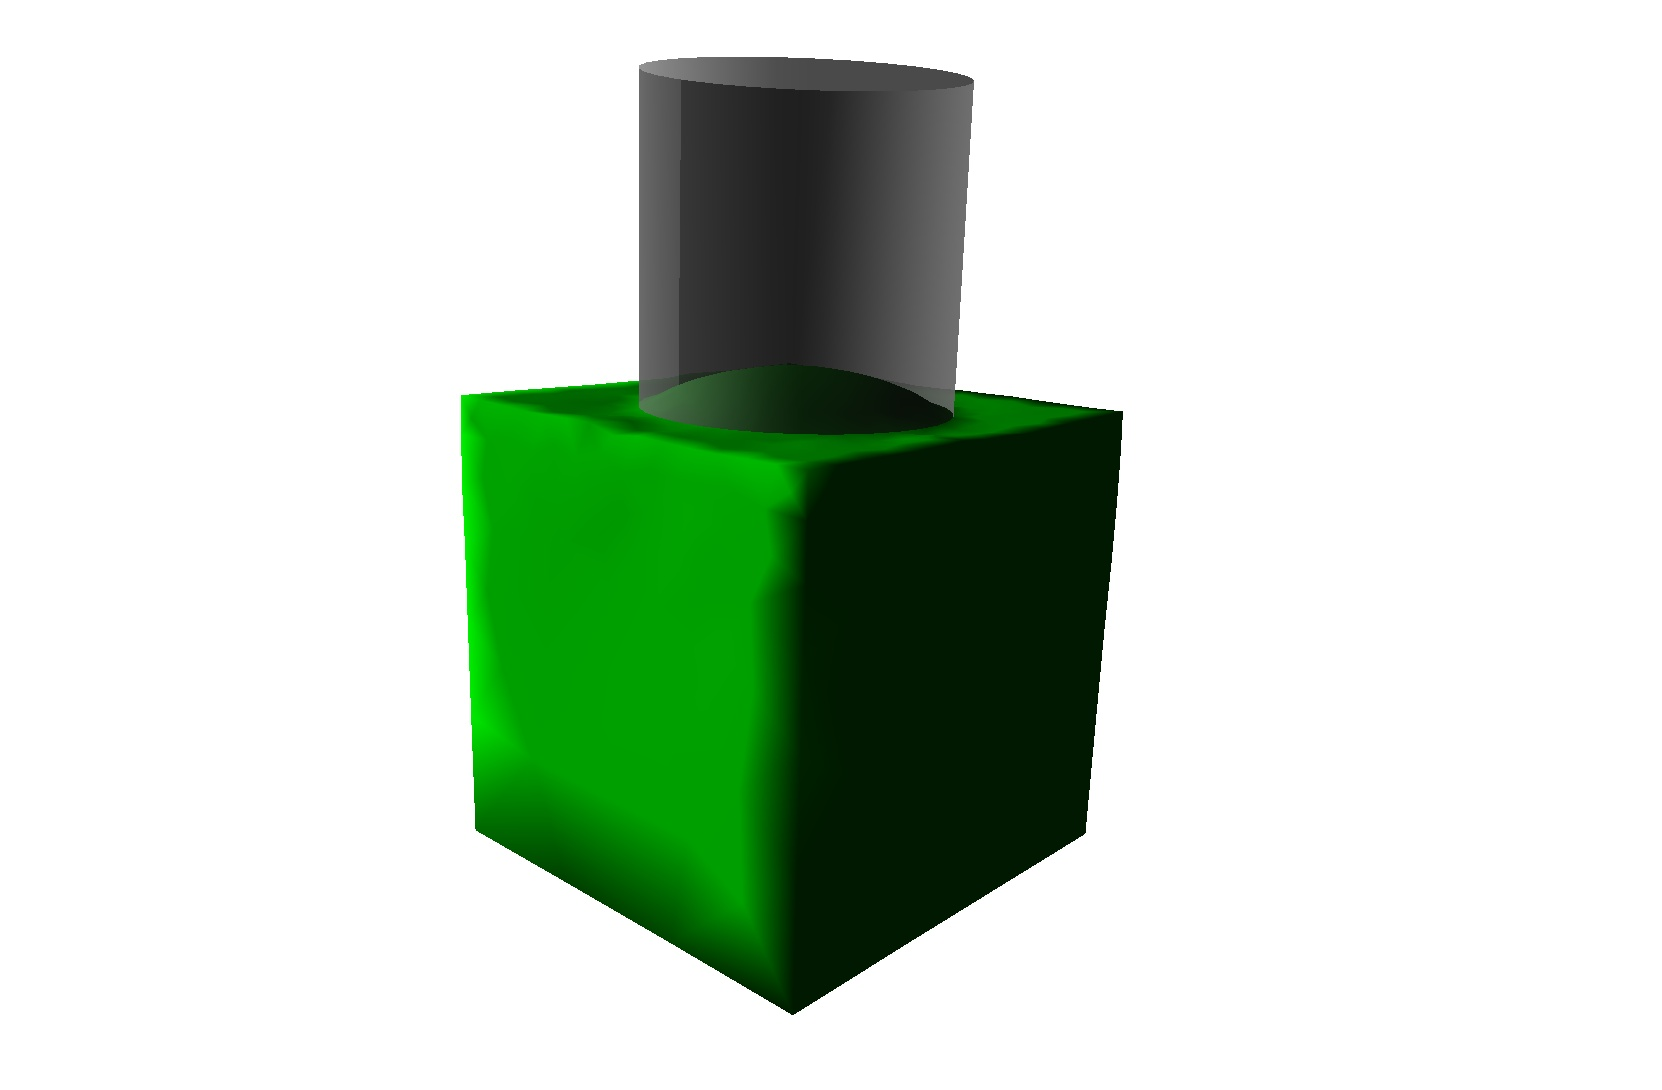
\includegraphics[height=3.5cm]{aspiration.jpg}}
	\subfigure[]{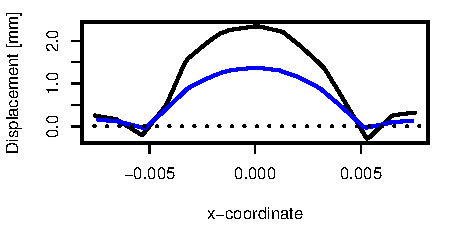
\includegraphics[width=7cm]{aspiration.pdf}}
  \caption{\label{fig-aspiration}Aspiration test: (a) the SOFA simulation scene, (b) displacment profile
  with (blue) and without (black) the capsule.}
\end{figure}

\subsection{Local Deformations} %{{{
During the contact with an instrument such as probe, needle, scalpel and others,
a specific deformations take place in the vicinity of
the instrument. This type of deformation may not necessarily induce the
deformation of the object as a whole and therefore can be considered as
local. Correct material properties are not only important to quantify the
displacement, but also play an important role in capturing the correct area of
the deformation or its profile near the instrument.

A good example of such a local deformation is the aspiration test
where the response of liver exposed locally to a negative pressure is measured.
In~\cite{Hollenstein2006} it is reported that the Glisson's
capsule has a non-negligible influence on the response of the tissue and modeling
only the parenchyma leads to an overestimation of the deformation. 
%We reproduced the test with our model and acquired similar results.
The aspiration device consists of a tube 1\,cm in diameter and is able
to control internal pressure in the tube. The test is performed by
attaching the tube to the tissue and measuring the tissue response. We
have set up a simulation in SOFA to reproduce the experiment (see Fig.~\ref{fig-aspiration}a: we meshed a 15$\times$15$\times$15\,mm$^3$ 
cube representing the tissue 
resulting in 2648 tetrahedra. Then we attached a 1\,cm tube 
and applied a pressure of 3\,kPa inside the tube. The interaction between the tube and 
tissue was modelled with friction contact. 

In Fig.~\ref{fig-aspiration}b the profiles of cuts in the middle of the
test cube are presented showing significantly larger deformation in the model without capsule. This is in perfect 
agreement with the results reported in~\cite{Hollenstein2006} and it can be concluded that 
our composite model based on coupling the triangular and tetrahedral elements provides an accurate 
model of parenchyma and capsule.

%}}}

\begin{figure}[t]
  \centering
    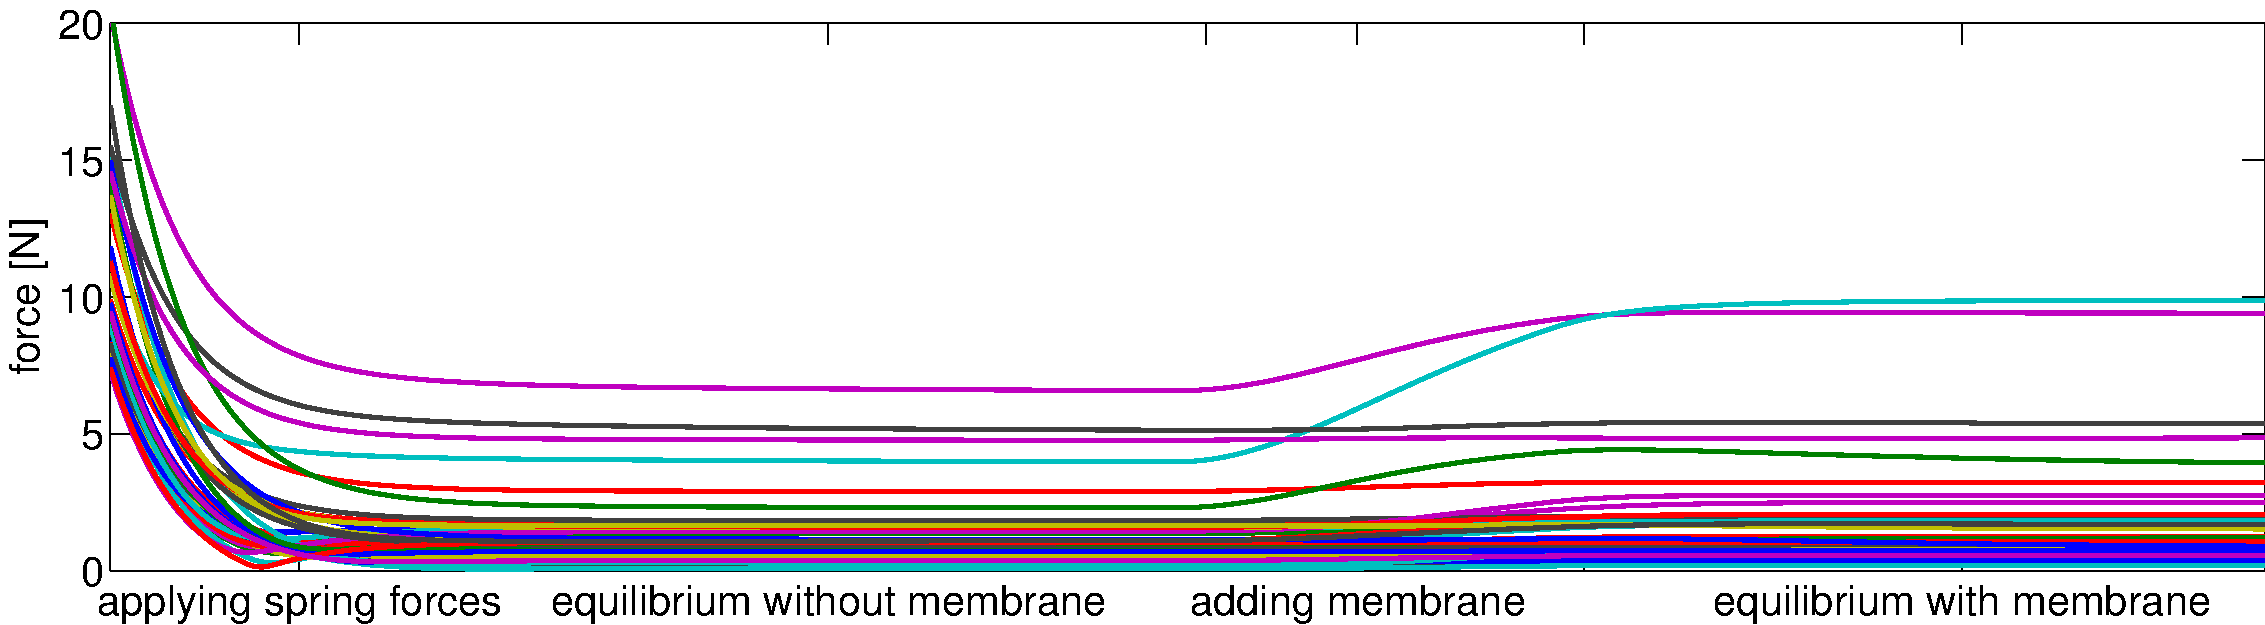
\includegraphics[width=.95\textwidth]{forceEvolution.pdf}
  \caption{\label{f:forceEvol}Evolution of forces during the simulation, where the supine data is deformed
towards the flank shape, and the stiffness of the capsule is increased from 0 to 8.22\,MPa after the initial equilibrium is achieved.}
\end{figure}

\subsection{Global Deformations}
In the previous section we have shown that the composite model of parenchyma and 
capsule can be used to reproduce the \emph{local} behaviour of the tissue. In the following, 
first we present a real-time complete model of entire liver built from image data. 
Second, using this model we demonstrate the \emph{global} mechanical influence of the capsule when 
the model undergoes large deformations. 

The complete model was constructed using contrast-enhanced CT data acquired on a female pig 
being positioned first in supine and then flank configuration. 
The liver and hepatic vein were segmented for both datasets  using semi-automatic methods available in ITKSnap~\footnote{www.itksnap.org}.
Further, an unstructured mesh was obtained from the segmented maps using CGAL~\footnote{www.cgal.org}. 
The semi-automatic method presented in~\cite{Peterlik2012} was 
then applied to the segmented map of the hepatic vein, resulting in linked-beam model. 
Finally, the model of the Glisson's capsule was constructed using the elements described in 
section~\ref{ss:capsuleModel} over the surface triangles extracted from the tetrahedral mesh. 
The complete model composed of 6200 tetrahedra, 220 beams and 1820 triangles was then 
used in simulation where external force representing the gravity was applied to the model, 
resulting in large deformations mainly in the area of lobes. The refresh rate of 10\,FPS 
was achieved on a desktop computer with Intel i7 CPU running at 3\,GHz and 16\,GB of memory. 
The simulation with gravity was also used as a first demonstration of the global influence of the capsule. 
In Fig.~\ref{f:global}a, the models with capsule (red) and without (yellow) are depicted after being 
deformed due to the gravity, showing a significant difference between the two models.  

\begin{figure}[t]
  \centering
    \subfigure[]{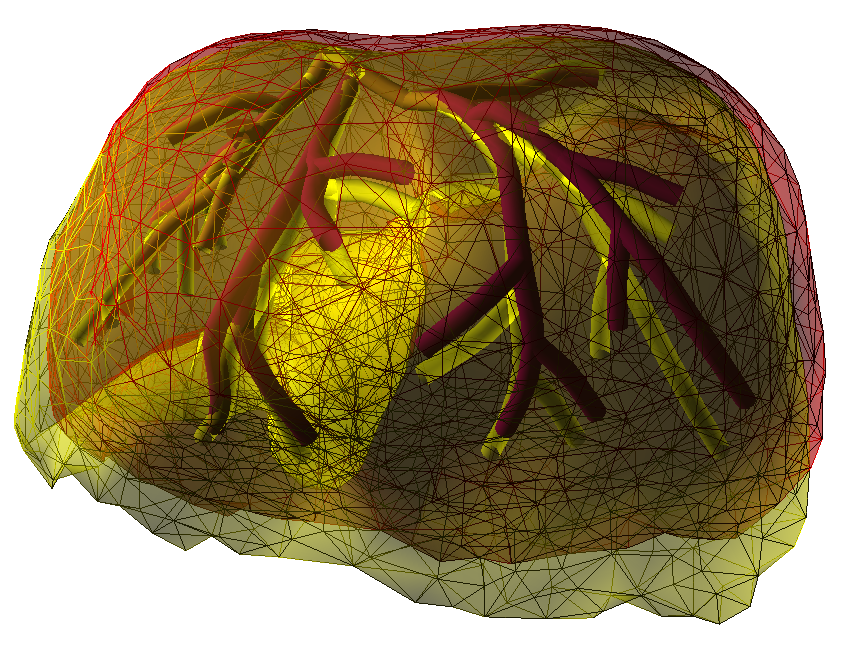
\includegraphics[width=.32\textwidth]{gravity2.png}}
    \subfigure[]{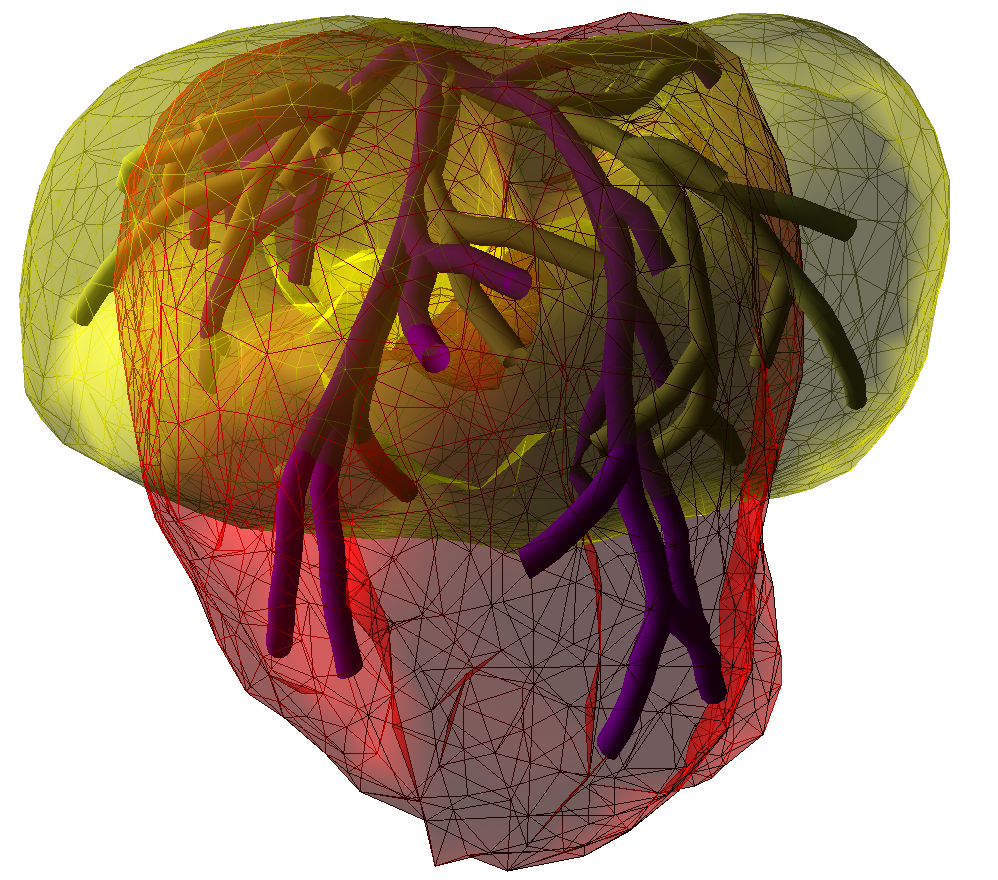
\includegraphics[width=.32\textwidth]{registered.png}}
    \subfigure[]{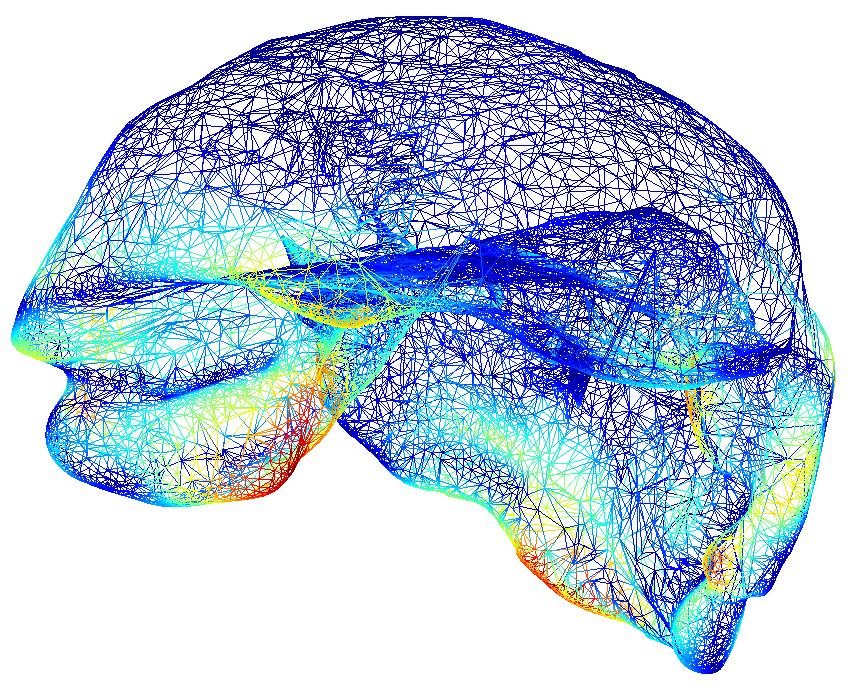
\includegraphics[width=.32\textwidth]{distanceMap.png}}
    \caption{\label{f:global}%
      (a) Liver under gravity with (red) and without (yellow) capsule;
      (b) liver in supine (yellow) and flank (red) position;
      (c) distance map between registered version with and without capsule.}
\end{figure}

In order to demonstrate the influence of the capsule on a real deformation of the liver, we 
performed a following protocol employing the supine and flank models built from the CT data. 
First, we performed a rigid registration of the two organs \wrt\ the root point of the hepatic vein. 
As shown in Fig.~\ref{f:global}b, the liver undergoes very large deformation when the body 
is turned from the supine to the flank position, exceeding 6\,cm for some parts of the organ. 
In order to induce similar deformation, we extracted feature pairs from the vascular system of the liver:
we selected points such as bifurcations which can be identified easily in both supine and flank 
data providing a set of correspondences. In the next step, we used these correspondences as a non-homogeneous
boundary conditions (imposed via penalty term) in order to perform a deformable registration of the supine
model onto the flank data. During the registration, the response forces acting in the points with prescribed displacements
were calculated. It is important to emphasize that the goal of the simulation was not 
to perform an accurate registration of the flank and supine data, but the simulation was used 
as an example of real deformation of the organ.

The simulation was performed with the model composed of parenchyma,  vessels and capsule, however, zero stiffness was 
set for the last component.
Once the static equilibrium was achieved, the effect of the capsule was gradually switched 
on, \ie\ the stiffness of the membrane was slowly increased from 0 to 8.22\,MPa. The evolution of the force response in the 
points with prescribed displacements is depicted in Fig.~\ref{f:forceEvol} showing the change in the response as the effect
of the capsule is included. At the same time, the shape of the deformed liver with capsule was compared 
to the model without the capsule. A distance map for those cases is depicted in Fig.~\ref{f:global}c: in the red areas, the 
maximal difference exceeding 1.5\,cm was measured. We believe that this result confirms that the Glisson's capsule 
plays an important role in the global mechanical response of the liver.

%}}}

\section{Conclusions} %{{{
In the paper, a complete model of the liver was presented taking into account 
three constituents of the organ, each being modelled with a different type 
of finite elements: tetrahedral corotational model used the parenchyma, serially 
linked corotational beams based on Tymoshenko formulation modelling the vascularization 
and finally triangular elements with constant strain employed for the capsule. 
The model was first validated for local displacements: the aspiration test presented in~\cite{Hollenstein2006} 
was successfully reproduced, showing a good agreement between the simulation and experiments. 
Further, the model was used to demonstrate global influence of the capsule when the organ 
undergoes large deformations. 

In the future work, we plan to employ the model to model other organs where the capsule play an important role
(for example kidneys). We will also focus on better understanding the interaction between the organs in the abdominal 
cavity. 

%While the influence of the capsule on local deformations was previously
%studied in the literature, it's significance on the global scale
%deformations of the liver remained unexplored. We have performed a set of
%natural global deformations of the complete liver and shown that the
%capsule, despite its small thickness, plays a significant role also in
%global context.
%
%}}}

%
% ---- Bibliography ----
%

\bibliographystyle{splncs03}
\bibliography{bibdata}


\end{document}
% spell: setl spell spelllang=en spellfile=spelldict.en.utf-8.add
% vim:set et sw=2 tw=75 fdm=marker fdl=3 fdc=4 isk+=_,-:
